% Author: Davide Armenante

\documentclass[fleqn]{article}
% Homework structure file

%___________________________________________________________________________________
% Packages
\usepackage[british]{babel}

\usepackage[margin=2.54cm]{geometry}

\usepackage{amsfonts,amsmath,amssymb}

\usepackage[none]{hyphenat}

\usepackage{fancyhdr}

\usepackage{booktabs}

\usepackage{graphicx}

\usepackage{float}

\usepackage{parskip}

\usepackage{subcaption}

\usepackage{amsmath}

\usepackage{wrapfig}

\usepackage{multicol}

\usepackage{chngcntr}

\counterwithin{figure}{section}

\counterwithin{equation}{section}

\usepackage[official]{eurosym}

\usepackage{gensymb}

\usepackage{listings}

\usepackage{color} %red, green, blue, yellow, cyan, magenta, black, white

%___________________________________________________________________________________
% Definitions for code displaying

\definecolor{mygreen}{RGB}{0,168,0} % color values Red, Green, Blue
\definecolor{mylilas}{RGB}{170,55,241}

\lstset{language=Matlab,%
    %basicstyle=\color{red},
    breaklines=true,%
    morekeywords={matlab2tikz},
    keywordstyle=\color{blue},%
    morekeywords=[2]{1}, keywordstyle=[2]{\color{black}},
    identifierstyle=\color{black},%
    stringstyle=\color{mylilas},
    commentstyle=\color{mygreen},%
    showstringspaces=false,%without this there will be a symbol in the places where there is a space
    numbers=left,%
    numberstyle={\tiny \color{black}},% size of the numbers
    numbersep=9pt, % this defines how far the numbers are from the text
    emph=[1]{for,end,break},emphstyle=[1]\color{red}, %some words to emphasise
    %emph=[2]{word1,word2}, emphstyle=[2]{style},    
}

%___________________________________________________________________________________
% Page Layout

\pagestyle{fancy}
\fancyhead{}
\fancyfoot{}
\fancyhead[L]{\slshape \MakeUppercase{Homeworks}}
\fancyhead[R]{\slshape Davide Armenante}
\fancyfoot[C]{\thepage}

\begin{document}

\begin{titlepage}
	\begin{center}
		\vspace{1cm}
		\large{\textbf{UNIVERSITA DEGLI STUDI DI TRIESTE}}\\[3mm]
		\large{\textbf{Dipartimento di Ingegneria e Architettura}}\\[.7mm]
		\large{\textbf{Corso di studi in Ingegneria Meccanica}}\\
		\begin{figure}
			\centering
			  
\includegraphics[width=3cm]{fig/unilogo.pdf}
		\end{figure}
		\vfill
		\line(1,0){400}\\
		\huge{\textbf{Esercitazioni}}\\
		\line(1,0){400}\\
		\vfill
		\hfill \normalsize Davide Armenante\\
		\line(1,0){400}\\
		Anno Accademico 2019-2020
		
	\end{center}
\end{titlepage}

\pagebreak
\tableofcontents 
\thispagestyle{empty}
\pagebreak
\setcounter{page}{1}

\section{Esercitazione - 17/03/2020}
La variazione del coefficiente di resistenza è non banale, dipende sia dal numero di Reynolds che dalla rugosità del filo. Abbiamo tranquillamente un errore del 50 perc se non si tiene conto della rugosità.

Il problema è il seguente. Dato lo chassis di una vettura da corsa i vede che le baRre di torsione sono cilindriche, si vuole costruire una carenatura in modo da rendere minima la resistenza aerodinamica. 
\begin{table}[h!]
\centering
\begin{tabular}{cccc}
\toprule
\begin{tabular}[c]{@{}c@{}}$\boldsymbol{T}$\\ $[K]$\end{tabular} & \begin{tabular}[c]{@{}c@{}}$\boldsymbol{\rho}$\\ $[kg/m^3]$\end{tabular} & \begin{tabular}[c]{@{}c@{}}$\boldsymbol{\mu}$\\ $[Pa \cdot s]$\end{tabular} & \begin{tabular}[c]{@{}c@{}}$\boldsymbol{a}$\\ $[m/s]$\end{tabular} \\
\midrule
$288.15$                                                         & $1.2250$                                                                 & $1.79 \cdot 10^{-5}$  
                                                  & $340.29$                                                          \\
\bottomrule       
\end{tabular}
\caption{Proprietà dell'aria}
\label{tab:Prop}
\end{table}
\begin{table}[h!]
\centering
\begin{tabular}{ccc}
\toprule
\begin{tabular}[c]{@{}c@{}}$\boldsymbol{d}$\\ $[mm]$\end{tabular} & \begin{tabular}[c]{@{}c@{}}$\boldsymbol{V}$\\ $[km/h]$\end{tabular} & \begin{tabular}[c]{@{}c@{}}$\boldsymbol{L}$\\ $[m]$\end{tabular} \\
\midrule
$25$                                                              & $320$                                                               & $1$                                                             \\
\bottomrule
\end{tabular}
\caption{Dati del problema}
\label{tab:dati}
\end{table}
Bisogna costruire un profilo aerodinamico attorno al profilo cilindrico (Figura \ref{fig:NACA0012}).
Si parte inserendo la sezione cilindrica in un profilo NACA0012. 
Si usano le condizioni standard per l'aria.
\begin{figure}[h!]
\centering
  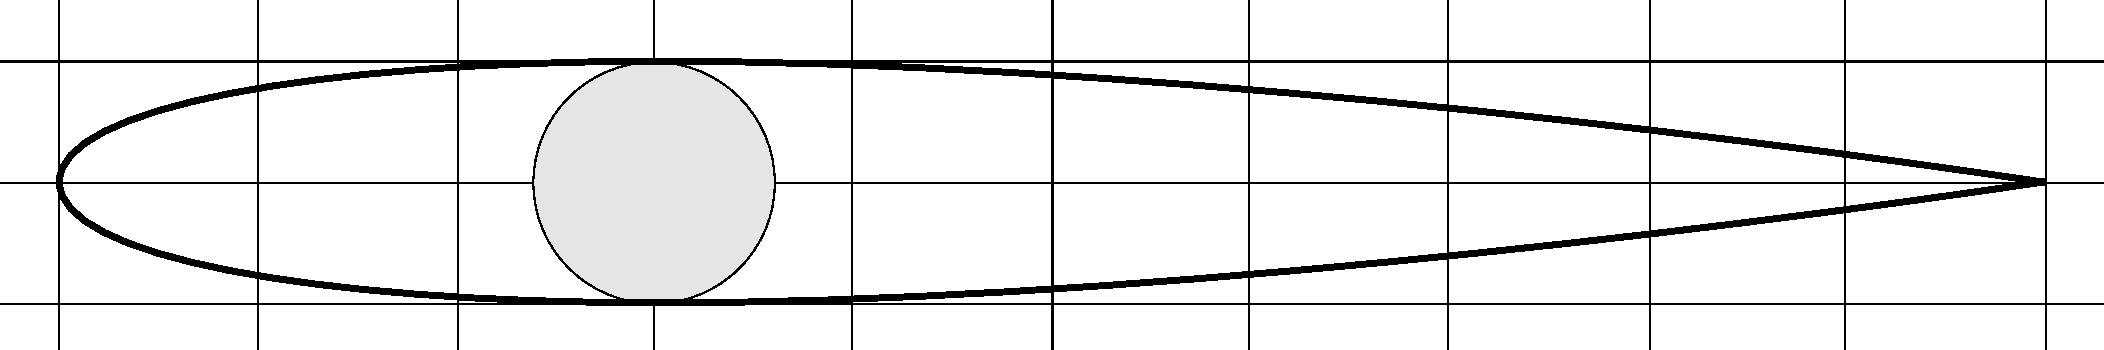
\includegraphics[width=.7\textwidth]{fig/NACA0012.pdf}
\caption{}
\label{fig:NACA0012}
\end{figure} 

Per il cilindro si avrà
\begin{align*}
Re = \frac{\rho V d}{\mu} = 1.52 \cdot 10^5
\end{align*}
\begin{align*}
Ma = \frac{V}{a} = 0.26
\end{align*}

Entrando nel diagramma in Figura \ref{fig:cW} ottengo il coefficiente $c_W = c_D = 1.25$ posso quindi calcolarmi la forza di drag
\begin{align*}
W = \frac{1}{2} \rho V_{\infty}^2 dl c_D = 151 \; N
\end{align*}

NACA0012, il profilo è il $12\%$ della corda. MP sono coefficienti della curva di 4 grado e sono indici di curvatura.

Nei profili aerodinamici $Re$ è calcolato rispetto alla corda, si avrà quindi 
\begin{align*}
c = \frac{d}{0.12} = 0.208 m 
\end{align*}
Quindi
\begin{align*}
Re =  \frac{\rho V c}{\mu} \simeq 1.27 \cdot 10^6
\end{align*}
Posso quindi usare il diagramma con $Re = 3 \cdot 10^6$ per la determinazione del coefficiente di drag del profilo alare $c_D = 0.005$ per $\alpha = 0$.
In questo caso il drag vale 
\begin{align*}
D = c_D \cdot \frac{1}{2} \cdot \rho \cdot V^2 \cdot c \cdot L  = 5.04 \; N
\end{align*}

Valori che confrontati con il valori precedenti sono drasticamente più bassi. 
Questa operazione può essere fatta utilizzando uno strumento di calcolo più sofisticato. Bisogna fare un workflow dentro modfroindier che lanscia xfoil e minimizza il drag. Il profilo ottimale è un NACA0012, 0010 o che altro?
\begin{figure}
\centering
  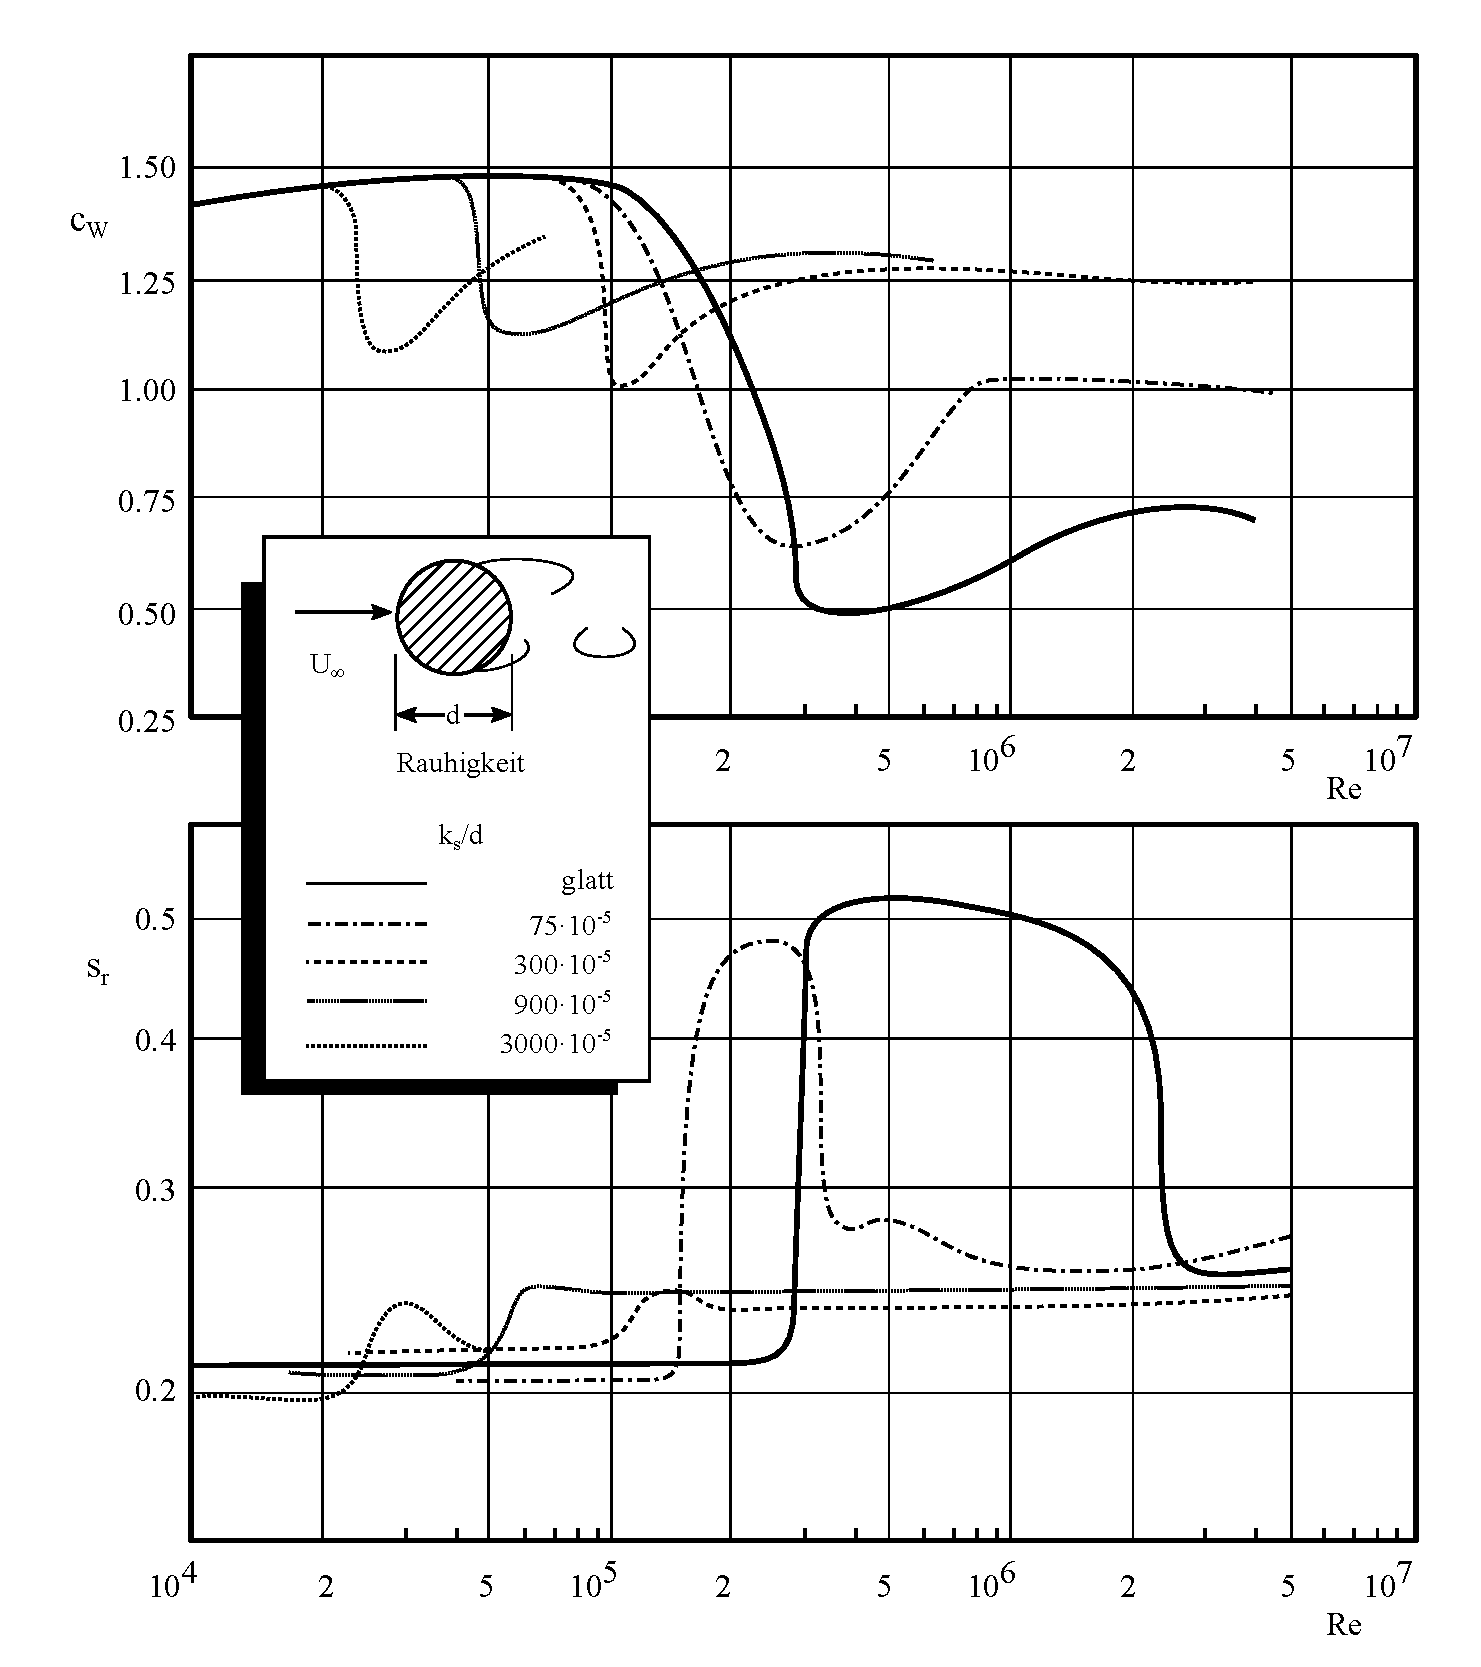
\includegraphics[width=\textwidth]{fig/coefficienteW.pdf}
\caption{}
\label{fig:cW}
\end{figure} 
\begin{figure}
\centering
  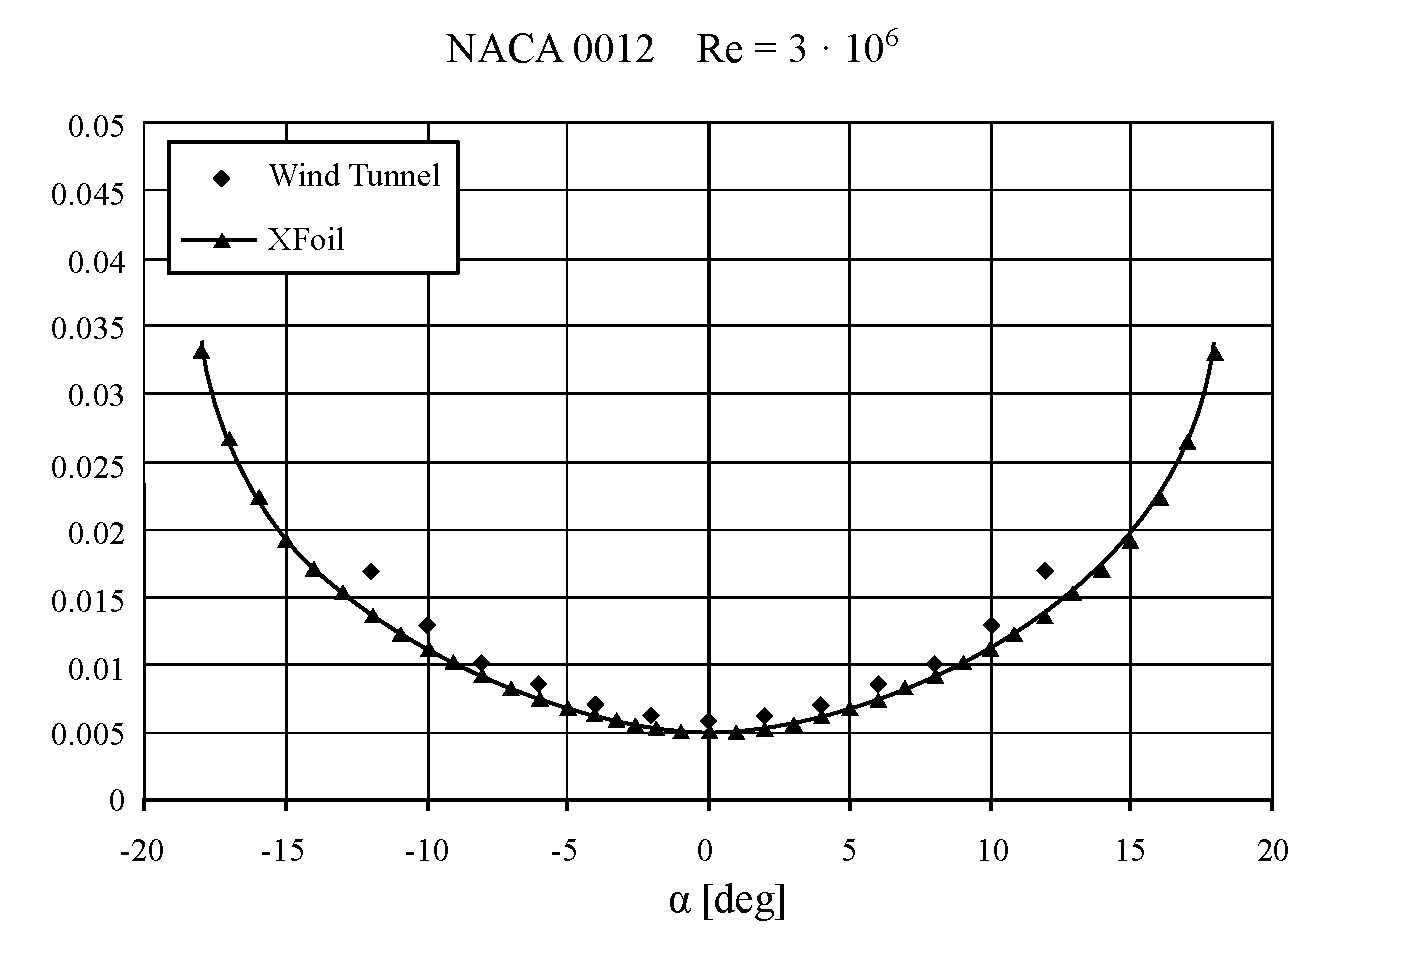
\includegraphics[width=\textwidth]{fig/DragCoeffXFOIL.pdf}
\caption{}
\label{fig:cW}
\end{figure} 
\end{document}

Si tratta di scrivere una geometria sotto forma di segmenti di curve polinomiali controllate in modo da mantenere o le curvature o le continuità. Nel caso di forme aerodinamiche ci sono 2 apsetti importanti. Bisogna mantenere la continuità dei unti (geometria chiusa), mantenere la derivata prima e spesso nel caso di flusso comprimibile mantenere la continuità di derivata seconda. Derivata seconda continua significa accelerazione continua del flusso lungo il profilo, questo per evitare fenomeni come formazione di onde d'urto. 